\documentclass[1p]{elsarticle_modified}
%\bibliographystyle{elsarticle-num}

%\usepackage[colorlinks]{hyperref}
%\usepackage{abbrmath_seonhwa} %\Abb, \Ascr, \Acal ,\Abf, \Afrak
\usepackage{amsfonts}
\usepackage{amssymb}
\usepackage{amsmath}
\usepackage{amsthm}
\usepackage{scalefnt}
\usepackage{amsbsy}
\usepackage{kotex}
\usepackage{caption}
\usepackage{subfig}
\usepackage{color}
\usepackage{graphicx}
\usepackage{xcolor} %% white, black, red, green, blue, cyan, magenta, yellow
\usepackage{float}
\usepackage{setspace}
\usepackage{hyperref}

\usepackage{tikz}
\usetikzlibrary{arrows}

\usepackage{multirow}
\usepackage{array} % fixed length table
\usepackage{hhline}

%%%%%%%%%%%%%%%%%%%%%
\makeatletter
\renewcommand*\env@matrix[1][\arraystretch]{%
	\edef\arraystretch{#1}%
	\hskip -\arraycolsep
	\let\@ifnextchar\new@ifnextchar
	\array{*\c@MaxMatrixCols c}}
\makeatother %https://tex.stackexchange.com/questions/14071/how-can-i-increase-the-line-spacing-in-a-matrix
%%%%%%%%%%%%%%%

\usepackage[normalem]{ulem}

\newcommand{\msout}[1]{\ifmmode\text{\sout{\ensuremath{#1}}}\else\sout{#1}\fi}
%SOURCE: \msout is \stkout macro in https://tex.stackexchange.com/questions/20609/strikeout-in-math-mode

\newcommand{\cancel}[1]{
	\ifmmode
	{\color{red}\msout{#1}}
	\else
	{\color{red}\sout{#1}}
	\fi
}

\newcommand{\add}[1]{
	{\color{blue}\uwave{#1}}
}

\newcommand{\replace}[2]{
	\ifmmode
	{\color{red}\msout{#1}}{\color{blue}\uwave{#2}}
	\else
	{\color{red}\sout{#1}}{\color{blue}\uwave{#2}}
	\fi
}

\newcommand{\Sol}{\mathcal{S}} %segment
\newcommand{\D}{D} %diagram
\newcommand{\A}{\mathcal{A}} %arc


%%%%%%%%%%%%%%%%%%%%%%%%%%%%%5 test

\def\sl{\operatorname{\textup{SL}}(2,\Cbb)}
\def\psl{\operatorname{\textup{PSL}}(2,\Cbb)}
\def\quan{\mkern 1mu \triangleright \mkern 1mu}

\theoremstyle{definition}
\newtheorem{thm}{Theorem}[section]
\newtheorem{prop}[thm]{Proposition}
\newtheorem{lem}[thm]{Lemma}
\newtheorem{ques}[thm]{Question}
\newtheorem{cor}[thm]{Corollary}
\newtheorem{defn}[thm]{Definition}
\newtheorem{exam}[thm]{Example}
\newtheorem{rmk}[thm]{Remark}
\newtheorem{alg}[thm]{Algorithm}

\newcommand{\I}{\sqrt{-1}}
\begin{document}

%\begin{frontmatter}
%
%\title{Boundary parabolic representations of knots up to 8 crossings}
%
%%% Group authors per affiliation:
%\author{Yunhi Cho} 
%\address{Department of Mathematics, University of Seoul, Seoul, Korea}
%\ead{yhcho@uos.ac.kr}
%
%
%\author{Seonhwa Kim} %\fnref{s_kim}}
%\address{Center for Geometry and Physics, Institute for Basic Science, Pohang, 37673, Korea}
%\ead{ryeona17@ibs.re.kr}
%
%\author{Hyuk Kim}
%\address{Department of Mathematical Sciences, Seoul National University, Seoul 08826, Korea}
%\ead{hyukkim@snu.ac.kr}
%
%\author{Seokbeom Yoon}
%\address{Department of Mathematical Sciences, Seoul National University, Seoul, 08826,  Korea}
%\ead{sbyoon15@snu.ac.kr}
%
%\begin{abstract}
%We find all boundary parabolic representation of knots up to 8 crossings.
%
%\end{abstract}
%\begin{keyword}
%    \MSC[2010] 57M25 
%\end{keyword}
%
%\end{frontmatter}

%\linenumbers
%\tableofcontents
%
\newcommand\colored[1]{\textcolor{white}{\rule[-0.35ex]{0.8em}{1.4ex}}\kern-0.8em\color{red} #1}%
%\newcommand\colored[1]{\textcolor{white}{ #1}\kern-2.17ex	\textcolor{white}{ #1}\kern-1.81ex	\textcolor{white}{ #1}\kern-2.15ex\color{red}#1	}

{\Large $\underline{12n_{0041}~(K12n_{0041})}$}

\setlength{\tabcolsep}{10pt}
\renewcommand{\arraystretch}{1.6}
\vspace{1cm}\begin{tabular}{m{100pt}>{\centering\arraybackslash}m{274pt}}
\multirow{5}{120pt}{
	\centering
	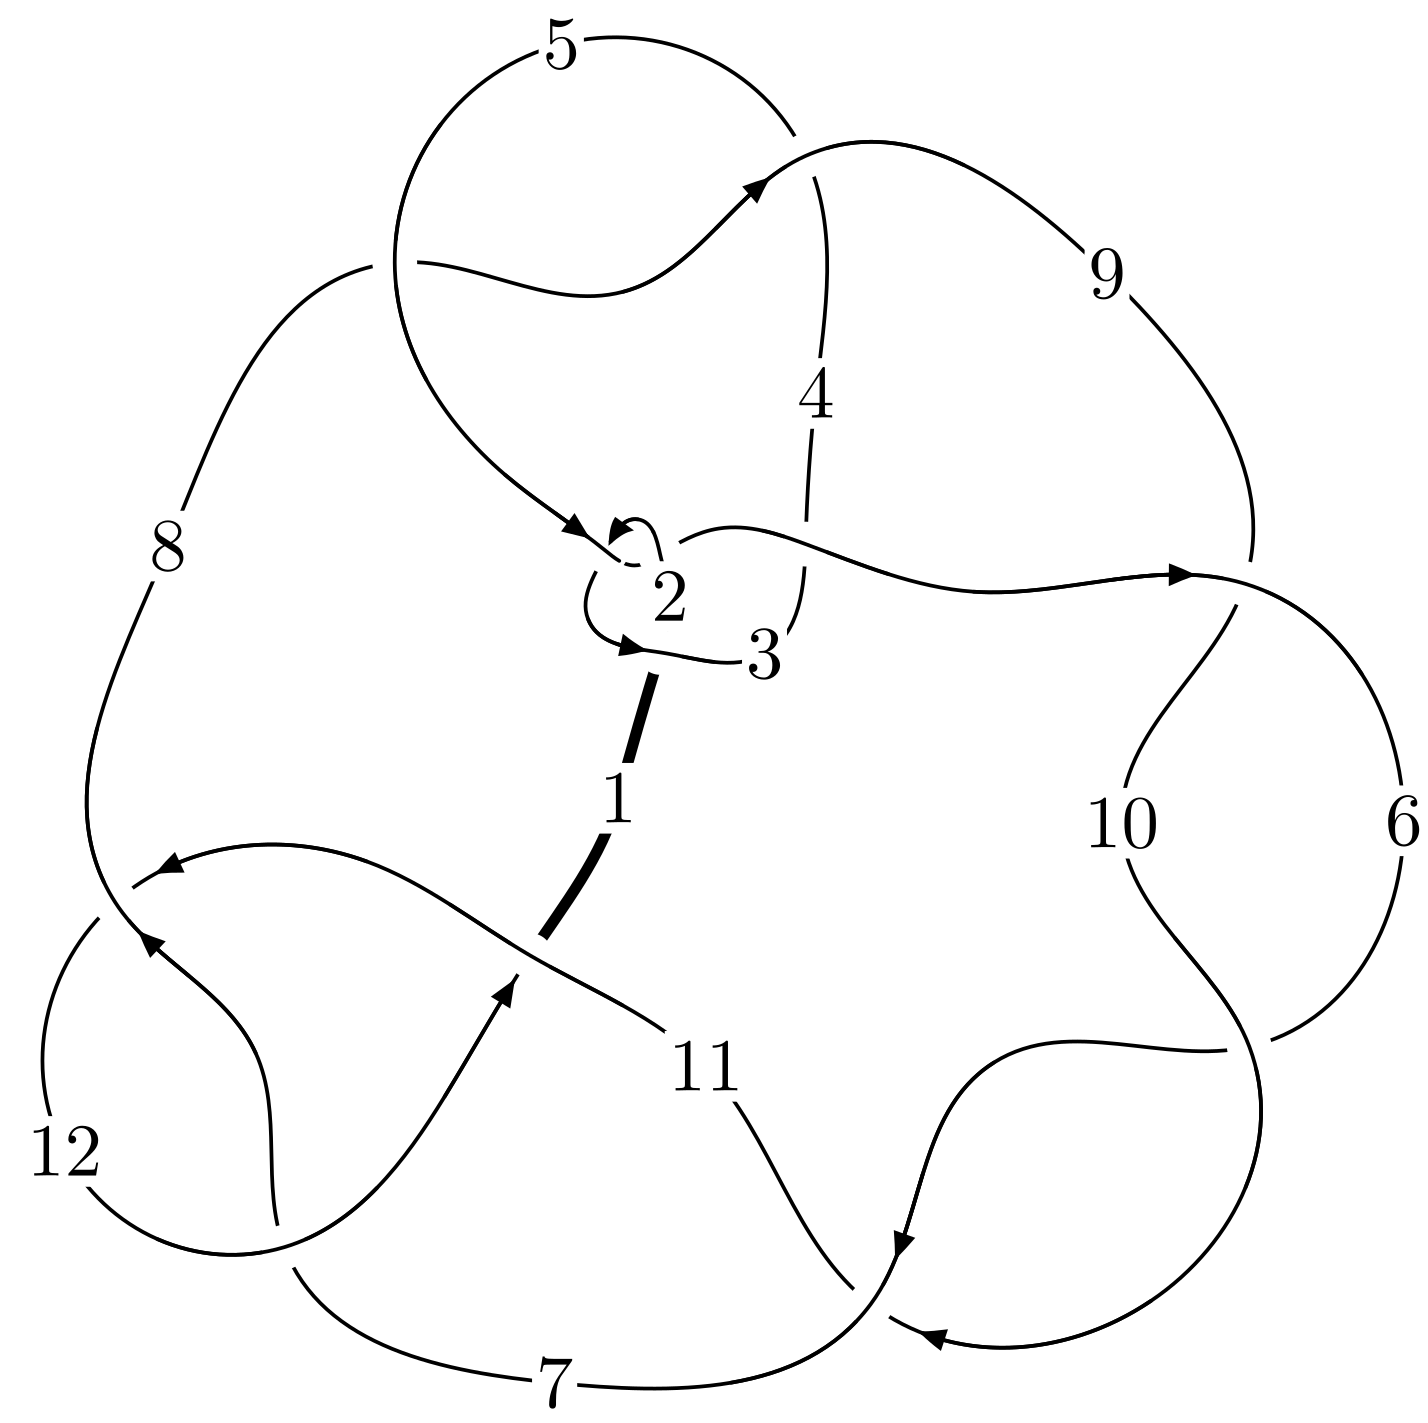
\includegraphics[width=112pt]{../../../GIT/diagram.site/Diagrams/png/2130_12n_0041.png}\\
\ \ \ A knot diagram\footnotemark}&
\allowdisplaybreaks
\textbf{Linearized knot diagam} \\
\cline{2-2}
 &
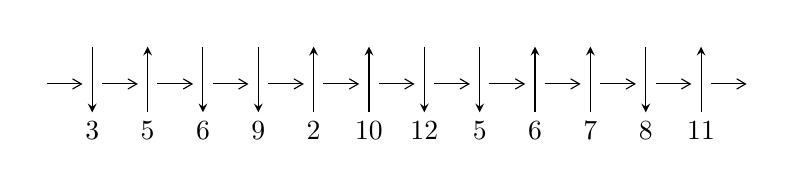
\begin{tikzpicture}[x=20pt, y=17pt]
	% nodes
	\node (C0) at (0, 0) {};
	\node (C1) at (1, 0) {};
	\node (C1U) at (1, +1) {};
	\node (C1D) at (1, -1) {3};

	\node (C2) at (2, 0) {};
	\node (C2U) at (2, +1) {};
	\node (C2D) at (2, -1) {5};

	\node (C3) at (3, 0) {};
	\node (C3U) at (3, +1) {};
	\node (C3D) at (3, -1) {6};

	\node (C4) at (4, 0) {};
	\node (C4U) at (4, +1) {};
	\node (C4D) at (4, -1) {9};

	\node (C5) at (5, 0) {};
	\node (C5U) at (5, +1) {};
	\node (C5D) at (5, -1) {2};

	\node (C6) at (6, 0) {};
	\node (C6U) at (6, +1) {};
	\node (C6D) at (6, -1) {10};

	\node (C7) at (7, 0) {};
	\node (C7U) at (7, +1) {};
	\node (C7D) at (7, -1) {12};

	\node (C8) at (8, 0) {};
	\node (C8U) at (8, +1) {};
	\node (C8D) at (8, -1) {5};

	\node (C9) at (9, 0) {};
	\node (C9U) at (9, +1) {};
	\node (C9D) at (9, -1) {6};

	\node (C10) at (10, 0) {};
	\node (C10U) at (10, +1) {};
	\node (C10D) at (10, -1) {7};

	\node (C11) at (11, 0) {};
	\node (C11U) at (11, +1) {};
	\node (C11D) at (11, -1) {8};

	\node (C12) at (12, 0) {};
	\node (C12U) at (12, +1) {};
	\node (C12D) at (12, -1) {11};
	\node (C13) at (13, 0) {};

	% arrows
	\draw[->,>={angle 60}]
	(C0) edge (C1) (C1) edge (C2) (C2) edge (C3) (C3) edge (C4) (C4) edge (C5) (C5) edge (C6) (C6) edge (C7) (C7) edge (C8) (C8) edge (C9) (C9) edge (C10) (C10) edge (C11) (C11) edge (C12) (C12) edge (C13) ;	\draw[->,>=stealth]
	(C1U) edge (C1D) (C2D) edge (C2U) (C3U) edge (C3D) (C4U) edge (C4D) (C5D) edge (C5U) (C6D) edge (C6U) (C7U) edge (C7D) (C8U) edge (C8D) (C9D) edge (C9U) (C10D) edge (C10U) (C11U) edge (C11D) (C12D) edge (C12U) ;
	\end{tikzpicture} \\
\hhline{~~} \\& 
\textbf{Solving Sequence} \\ \cline{2-2} 
 &
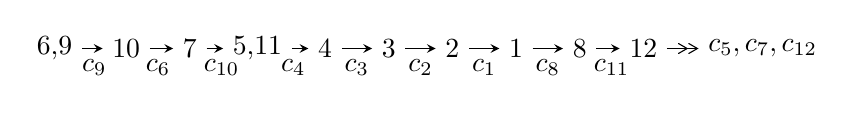
\begin{tikzpicture}[x=23pt, y=7pt]
	% node
	\node (A0) at (-1/8, 0) {6,9};
	\node (A1) at (1, 0) {10};
	\node (A2) at (2, 0) {7};
	\node (A3) at (49/16, 0) {5,11};
	\node (A4) at (33/8, 0) {4};
	\node (A5) at (41/8, 0) {3};
	\node (A6) at (49/8, 0) {2};
	\node (A7) at (57/8, 0) {1};
	\node (A8) at (65/8, 0) {8};
	\node (A9) at (73/8, 0) {12};
	\node (C1) at (1/2, -1) {$c_{9}$};
	\node (C2) at (3/2, -1) {$c_{6}$};
	\node (C3) at (5/2, -1) {$c_{10}$};
	\node (C4) at (29/8, -1) {$c_{4}$};
	\node (C5) at (37/8, -1) {$c_{3}$};
	\node (C6) at (45/8, -1) {$c_{2}$};
	\node (C7) at (53/8, -1) {$c_{1}$};
	\node (C8) at (61/8, -1) {$c_{8}$};
	\node (C9) at (69/8, -1) {$c_{11}$};
	\node (A10) at (11, 0) {$c_{5},c_{7},c_{12}$};

	% edge
	\draw[->,>=stealth]	
	(A0) edge (A1) (A1) edge (A2) (A2) edge (A3) (A3) edge (A4) (A4) edge (A5) (A5) edge (A6) (A6) edge (A7) (A7) edge (A8) (A8) edge (A9) ;
	\draw[->>,>={angle 60}]	
	(A9) edge (A10);
\end{tikzpicture} \\ 

\end{tabular} \\

\footnotetext{
The image of knot diagram is generated by the software ``\textbf{Draw programme}" developed by Andrew Bartholomew(\url{http://www.layer8.co.uk/maths/draw/index.htm\#Running-draw}), where we modified some parts for our purpose(\url{https://github.com/CATsTAILs/LinksPainter}).
}\phantom \\ \newline 
\centering \textbf{Ideals for irreducible components\footnotemark of $X_{\text{par}}$} 
 
\begin{align*}
I^u_{1}&=\langle 
801994252 u^{18}-3257723213 u^{17}+\cdots+1752268067 b+1712546026,\\
\phantom{I^u_{1}}&\phantom{= \langle  }-6711899247 u^{18}+18127971990 u^{17}+\cdots+3504536134 a+13273949042,\\
\phantom{I^u_{1}}&\phantom{= \langle  }u^{19}-3 u^{18}+\cdots+u-1\rangle \\
I^u_{2}&=\langle 
b,\;- u^4 a- u^3 a+u^4+2 u^2 a+2 u^3+a^2+a u- u^2- a-3 u,\;u^5+u^4-2 u^3- u^2+u-1\rangle \\
\\
\end{align*}
\raggedright * 2 irreducible components of $\dim_{\mathbb{C}}=0$, with total 29 representations.\\
\footnotetext{All coefficients of polynomials are rational numbers. But the coefficients are sometimes approximated in decimal forms when there is not enough margin.}
\newpage
\renewcommand{\arraystretch}{1}
\centering \section*{I. $I^u_{1}= \langle 8.02\times10^{8} u^{18}-3.26\times10^{9} u^{17}+\cdots+1.75\times10^{9} b+1.71\times10^{9},\;-6.71\times10^{9} u^{18}+1.81\times10^{10} u^{17}+\cdots+3.50\times10^{9} a+1.33\times10^{10},\;u^{19}-3 u^{18}+\cdots+u-1 \rangle$}
\flushleft \textbf{(i) Arc colorings}\\
\begin{tabular}{m{7pt} m{180pt} m{7pt} m{180pt} }
\flushright $a_{6}=$&$\begin{pmatrix}0\\u\end{pmatrix}$ \\
\flushright $a_{9}=$&$\begin{pmatrix}1\\0\end{pmatrix}$ \\
\flushright $a_{10}=$&$\begin{pmatrix}1\\- u^2\end{pmatrix}$ \\
\flushright $a_{7}=$&$\begin{pmatrix}u\\- u^3+u\end{pmatrix}$ \\
\flushright $a_{5}=$&$\begin{pmatrix}1.91520 u^{18}-5.17272 u^{17}+\cdots-4.28509 u-3.78765\\-0.457689 u^{18}+1.85915 u^{17}+\cdots-0.626511 u-0.977331\end{pmatrix}$ \\
\flushright $a_{11}=$&$\begin{pmatrix}- u^2+1\\u^4-2 u^2\end{pmatrix}$ \\
\flushright $a_{4}=$&$\begin{pmatrix}1.45751 u^{18}-3.31357 u^{17}+\cdots-4.91160 u-4.76498\\-0.457689 u^{18}+1.85915 u^{17}+\cdots-0.626511 u-0.977331\end{pmatrix}$ \\
\flushright $a_{3}=$&$\begin{pmatrix}1.45751 u^{18}-3.31357 u^{17}+\cdots-4.91160 u-4.76498\\-0.744876 u^{18}+2.99066 u^{17}+\cdots-1.02505 u-2.03630\end{pmatrix}$ \\
\flushright $a_{2}=$&$\begin{pmatrix}0.688639 u^{18}-1.66148 u^{17}+\cdots+1.68347 u-4.87205\\-0.257833 u^{18}+0.974337 u^{17}+\cdots+0.715799 u-0.404438\end{pmatrix}$ \\
\flushright $a_{1}=$&$\begin{pmatrix}-1.18863 u^{18}+4.77080 u^{17}+\cdots-1.55380 u-4.47346\\-0.835657 u^{18}+2.70331 u^{17}+\cdots+4.20709 u-3.06916\end{pmatrix}$ \\
\flushright $a_{8}=$&$\begin{pmatrix}-1.86427 u^{18}+5.34890 u^{17}+\cdots+2.46844 u-0.0507078\\-1.20490 u^{18}+3.02293 u^{17}+\cdots+3.28483 u+1.18863\end{pmatrix}$ \\
\flushright $a_{12}=$&$\begin{pmatrix}1.06187 u^{18}-4.23698 u^{17}+\cdots+1.50625 u+3.49695\\0.526384 u^{18}-1.72956 u^{17}+\cdots-3.80190 u+2.76211\end{pmatrix}$\\&\end{tabular}
\flushleft \textbf{(ii) Obstruction class $= -1$}\\~\\
\flushleft \textbf{(iii) Cusp Shapes $= \frac{3543125147}{3504536134} u^{18}-\frac{342620995}{3504536134} u^{17}+\cdots-\frac{5030153644}{159297097} u-\frac{4276661878}{1752268067}$}\\~\\
\newpage\renewcommand{\arraystretch}{1}
\flushleft \textbf{(iv) u-Polynomials at the component}\newline \\
\begin{tabular}{m{50pt}|m{274pt}}
Crossings & \hspace{64pt}u-Polynomials at each crossing \\
\hline $$\begin{aligned}c_{1}\end{aligned}$$&$\begin{aligned}
&u^{19}+22 u^{17}+\cdots-12 u-1
\end{aligned}$\\
\hline $$\begin{aligned}c_{2},c_{5}\end{aligned}$$&$\begin{aligned}
&u^{19}+6 u^{18}+\cdots+4 u+1
\end{aligned}$\\
\hline $$\begin{aligned}c_{3}\end{aligned}$$&$\begin{aligned}
&u^{19}-6 u^{18}+\cdots+21156 u+4073
\end{aligned}$\\
\hline $$\begin{aligned}c_{4},c_{8}\end{aligned}$$&$\begin{aligned}
&u^{19}+u^{18}+\cdots-1024 u-1024
\end{aligned}$\\
\hline $$\begin{aligned}c_{6},c_{9},c_{10}\end{aligned}$$&$\begin{aligned}
&u^{19}-3 u^{18}+\cdots+u-1
\end{aligned}$\\
\hline $$\begin{aligned}c_{7},c_{11}\end{aligned}$$&$\begin{aligned}
&u^{19}+3 u^{18}+\cdots- u-1
\end{aligned}$\\
\hline $$\begin{aligned}c_{12}\end{aligned}$$&$\begin{aligned}
&u^{19}-13 u^{18}+\cdots-13 u+1
\end{aligned}$\\
\hline
\end{tabular}\\~\\
\newpage\renewcommand{\arraystretch}{1}
\flushleft \textbf{(v) Riley Polynomials at the component}\newline \\
\begin{tabular}{m{50pt}|m{274pt}}
Crossings & \hspace{64pt}Riley Polynomials at each crossing \\
\hline $$\begin{aligned}c_{1}\end{aligned}$$&$\begin{aligned}
&y^{19}+44 y^{18}+\cdots-24 y-1
\end{aligned}$\\
\hline $$\begin{aligned}c_{2},c_{5}\end{aligned}$$&$\begin{aligned}
&y^{19}+22 y^{17}+\cdots-12 y-1
\end{aligned}$\\
\hline $$\begin{aligned}c_{3}\end{aligned}$$&$\begin{aligned}
&y^{19}+88 y^{18}+\cdots-418750764 y-16589329
\end{aligned}$\\
\hline $$\begin{aligned}c_{4},c_{8}\end{aligned}$$&$\begin{aligned}
&y^{19}+55 y^{18}+\cdots-1048576 y-1048576
\end{aligned}$\\
\hline $$\begin{aligned}c_{6},c_{9},c_{10}\end{aligned}$$&$\begin{aligned}
&y^{19}-35 y^{18}+\cdots-13 y-1
\end{aligned}$\\
\hline $$\begin{aligned}c_{7},c_{11}\end{aligned}$$&$\begin{aligned}
&y^{19}+13 y^{18}+\cdots-13 y-1
\end{aligned}$\\
\hline $$\begin{aligned}c_{12}\end{aligned}$$&$\begin{aligned}
&y^{19}-11 y^{18}+\cdots-13 y-1
\end{aligned}$\\
\hline
\end{tabular}\\~\\
\newpage\flushleft \textbf{(vi) Complex Volumes and Cusp Shapes}
$$\begin{array}{c|c|c}  
\text{Solutions to }I^u_{1}& \I (\text{vol} + \sqrt{-1}CS) & \text{Cusp shape}\\
 \hline 
\begin{aligned}
u &= \phantom{-}0.469936 + 0.580822 I \\
a &= -0.046125 - 0.179882 I \\
b &= \phantom{-}0.481085 + 0.331499 I\end{aligned}
 & \phantom{-}0.32482 + 1.95207 I & \phantom{-}0.24383 - 3.23848 I \\ \hline\begin{aligned}
u &= \phantom{-}0.469936 - 0.580822 I \\
a &= -0.046125 + 0.179882 I \\
b &= \phantom{-}0.481085 - 0.331499 I\end{aligned}
 & \phantom{-}0.32482 - 1.95207 I & \phantom{-}0.24383 + 3.23848 I \\ \hline\begin{aligned}
u &= \phantom{-}0.203301 + 0.528628 I \\
a &= \phantom{-}1.67634 + 1.79943 I \\
b &= \phantom{-}1.52335 + 0.99869 I\end{aligned}
 & \phantom{-}3.95992 - 1.78665 I & \phantom{-}6.73687 + 1.96158 I \\ \hline\begin{aligned}
u &= \phantom{-}0.203301 - 0.528628 I \\
a &= \phantom{-}1.67634 - 1.79943 I \\
b &= \phantom{-}1.52335 - 0.99869 I\end{aligned}
 & \phantom{-}3.95992 + 1.78665 I & \phantom{-}6.73687 - 1.96158 I \\ \hline\begin{aligned}
u &= \phantom{-}0.008315 + 0.564548 I \\
a &= -0.357902 - 0.497669 I \\
b &= -0.424228 + 0.518164 I\end{aligned}
 & -0.40680 + 1.36117 I & -2.67817 - 4.58018 I \\ \hline\begin{aligned}
u &= \phantom{-}0.008315 - 0.564548 I \\
a &= -0.357902 + 0.497669 I \\
b &= -0.424228 - 0.518164 I\end{aligned}
 & -0.40680 - 1.36117 I & -2.67817 + 4.58018 I \\ \hline\begin{aligned}
u &= -0.501281 + 0.026931 I \\
a &= -1.86678 - 2.02772 I \\
b &= -0.171729 + 1.042670 I\end{aligned}
 & \phantom{-}1.56074 - 3.66143 I & \phantom{-}5.39141 + 4.20256 I \\ \hline\begin{aligned}
u &= -0.501281 - 0.026931 I \\
a &= -1.86678 + 2.02772 I \\
b &= -0.171729 - 1.042670 I\end{aligned}
 & \phantom{-}1.56074 + 3.66143 I & \phantom{-}5.39141 - 4.20256 I \\ \hline\begin{aligned}
u &= \phantom{-}1.56360\phantom{ +0.000000I} \\
a &= -0.443721\phantom{ +0.000000I} \\
b &= \phantom{-}1.34603\phantom{ +0.000000I}\end{aligned}
 & \phantom{-}3.65542\phantom{ +0.000000I} & \phantom{-}2.34160\phantom{ +0.000000I} \\ \hline\begin{aligned}
u &= \phantom{-}0.111360 + 0.361359 I \\
a &= -1.08886 - 1.51643 I \\
b &= -0.369696 + 0.488600 I\end{aligned}
 & -0.21591 + 1.44599 I & -1.60179 - 5.31059 I\\
 \hline 
 \end{array}$$\newpage$$\begin{array}{c|c|c}  
\text{Solutions to }I^u_{1}& \I (\text{vol} + \sqrt{-1}CS) & \text{Cusp shape}\\
 \hline 
\begin{aligned}
u &= \phantom{-}0.111360 - 0.361359 I \\
a &= -1.08886 + 1.51643 I \\
b &= -0.369696 - 0.488600 I\end{aligned}
 & -0.21591 - 1.44599 I & -1.60179 + 5.31059 I \\ \hline\begin{aligned}
u &= -1.72009 + 0.19693 I \\
a &= \phantom{-}0.513343 - 0.171232 I \\
b &= -1.51868 + 0.49853 I\end{aligned}
 & \phantom{-}7.40108 - 4.89405 I & \phantom{-}5.57785 + 2.97654 I \\ \hline\begin{aligned}
u &= -1.72009 - 0.19693 I \\
a &= \phantom{-}0.513343 + 0.171232 I \\
b &= -1.51868 - 0.49853 I\end{aligned}
 & \phantom{-}7.40108 + 4.89405 I & \phantom{-}5.57785 - 2.97654 I \\ \hline\begin{aligned}
u &= \phantom{-}2.15399 + 0.20015 I \\
a &= -0.240429 - 1.266600 I \\
b &= -0.26878 + 3.56600 I\end{aligned}
 & -15.5249 - 1.2175 I & \phantom{-}5.22163 + 0.77720 I \\ \hline\begin{aligned}
u &= \phantom{-}2.15399 - 0.20015 I \\
a &= -0.240429 + 1.266600 I \\
b &= -0.26878 - 3.56600 I\end{aligned}
 & -15.5249 + 1.2175 I & \phantom{-}5.22163 - 0.77720 I \\ \hline\begin{aligned}
u &= \phantom{-}2.15940 + 0.15889 I \\
a &= \phantom{-}0.037600 - 1.236710 I \\
b &= -1.03657 + 3.06900 I\end{aligned}
 & -15.9786 + 9.8700 I & \phantom{-}4.75713 - 4.56429 I \\ \hline\begin{aligned}
u &= \phantom{-}2.15940 - 0.15889 I \\
a &= \phantom{-}0.037600 + 1.236710 I \\
b &= -1.03657 - 3.06900 I\end{aligned}
 & -15.9786 - 9.8700 I & \phantom{-}4.75713 + 4.56429 I \\ \hline\begin{aligned}
u &= -2.16674 + 0.18320 I \\
a &= \phantom{-}0.094666 - 1.203630 I \\
b &= \phantom{-}0.61224 + 3.16966 I\end{aligned}
 & \phantom{-}19.5194 - 4.2417 I & \phantom{-}2.18043 + 1.81116 I \\ \hline\begin{aligned}
u &= -2.16674 - 0.18320 I \\
a &= \phantom{-}0.094666 + 1.203630 I \\
b &= \phantom{-}0.61224 - 3.16966 I\end{aligned}
 & \phantom{-}19.5194 + 4.2417 I & \phantom{-}2.18043 - 1.81116 I\\
 \hline 
 \end{array}$$\newpage\newpage\renewcommand{\arraystretch}{1}
\centering \section*{II. $I^u_{2}= \langle b,\;- u^4 a+u^4+\cdots+a^2- a,\;u^5+u^4-2 u^3- u^2+u-1 \rangle$}
\flushleft \textbf{(i) Arc colorings}\\
\begin{tabular}{m{7pt} m{180pt} m{7pt} m{180pt} }
\flushright $a_{6}=$&$\begin{pmatrix}0\\u\end{pmatrix}$ \\
\flushright $a_{9}=$&$\begin{pmatrix}1\\0\end{pmatrix}$ \\
\flushright $a_{10}=$&$\begin{pmatrix}1\\- u^2\end{pmatrix}$ \\
\flushright $a_{7}=$&$\begin{pmatrix}u\\- u^3+u\end{pmatrix}$ \\
\flushright $a_{5}=$&$\begin{pmatrix}a\\0\end{pmatrix}$ \\
\flushright $a_{11}=$&$\begin{pmatrix}- u^2+1\\u^4-2 u^2\end{pmatrix}$ \\
\flushright $a_{4}=$&$\begin{pmatrix}a\\0\end{pmatrix}$ \\
\flushright $a_{3}=$&$\begin{pmatrix}a\\- u^2 a\end{pmatrix}$ \\
\flushright $a_{2}=$&$\begin{pmatrix}- u^4- u^3+2 u^2+a+u-1\\- u^2 a\end{pmatrix}$ \\
\flushright $a_{1}=$&$\begin{pmatrix}0\\- u\end{pmatrix}$ \\
\flushright $a_{8}=$&$\begin{pmatrix}1\\0\end{pmatrix}$ \\
\flushright $a_{12}=$&$\begin{pmatrix}- u^4+u^2+1\\u^4-2 u^2\end{pmatrix}$\\&\end{tabular}
\flushleft \textbf{(ii) Obstruction class $= 1$}\\~\\
\flushleft \textbf{(iii) Cusp Shapes $= u^4 a- u^4-2 u^2 a+2 u^3+3 a u+u^2+a-5 u+2$}\\~\\
\newpage\renewcommand{\arraystretch}{1}
\flushleft \textbf{(iv) u-Polynomials at the component}\newline \\
\begin{tabular}{m{50pt}|m{274pt}}
Crossings & \hspace{64pt}u-Polynomials at each crossing \\
\hline $$\begin{aligned}c_{1},c_{3},c_{5}\end{aligned}$$&$\begin{aligned}
&(u^2- u+1)^5
\end{aligned}$\\
\hline $$\begin{aligned}c_{2}\end{aligned}$$&$\begin{aligned}
&(u^2+u+1)^5
\end{aligned}$\\
\hline $$\begin{aligned}c_{4},c_{8}\end{aligned}$$&$\begin{aligned}
&u^{10}
\end{aligned}$\\
\hline $$\begin{aligned}c_{6}\end{aligned}$$&$\begin{aligned}
&(u^5- u^4-2 u^3+u^2+u+1)^2
\end{aligned}$\\
\hline $$\begin{aligned}c_{7}\end{aligned}$$&$\begin{aligned}
&(u^5+u^4+2 u^3+u^2+u+1)^2
\end{aligned}$\\
\hline $$\begin{aligned}c_{9},c_{10}\end{aligned}$$&$\begin{aligned}
&(u^5+u^4-2 u^3- u^2+u-1)^2
\end{aligned}$\\
\hline $$\begin{aligned}c_{11}\end{aligned}$$&$\begin{aligned}
&(u^5- u^4+2 u^3- u^2+u-1)^2
\end{aligned}$\\
\hline $$\begin{aligned}c_{12}\end{aligned}$$&$\begin{aligned}
&(u^5-3 u^4+4 u^3- u^2- u+1)^2
\end{aligned}$\\
\hline
\end{tabular}\\~\\
\newpage\renewcommand{\arraystretch}{1}
\flushleft \textbf{(v) Riley Polynomials at the component}\newline \\
\begin{tabular}{m{50pt}|m{274pt}}
Crossings & \hspace{64pt}Riley Polynomials at each crossing \\
\hline $$\begin{aligned}c_{1},c_{2},c_{3}\\c_{5}\end{aligned}$$&$\begin{aligned}
&(y^2+y+1)^5
\end{aligned}$\\
\hline $$\begin{aligned}c_{4},c_{8}\end{aligned}$$&$\begin{aligned}
&y^{10}
\end{aligned}$\\
\hline $$\begin{aligned}c_{6},c_{9},c_{10}\end{aligned}$$&$\begin{aligned}
&(y^5-5 y^4+8 y^3-3 y^2- y-1)^2
\end{aligned}$\\
\hline $$\begin{aligned}c_{7},c_{11}\end{aligned}$$&$\begin{aligned}
&(y^5+3 y^4+4 y^3+y^2- y-1)^2
\end{aligned}$\\
\hline $$\begin{aligned}c_{12}\end{aligned}$$&$\begin{aligned}
&(y^5- y^4+8 y^3-3 y^2+3 y-1)^2
\end{aligned}$\\
\hline
\end{tabular}\\~\\
\newpage\flushleft \textbf{(vi) Complex Volumes and Cusp Shapes}
$$\begin{array}{c|c|c}  
\text{Solutions to }I^u_{2}& \I (\text{vol} + \sqrt{-1}CS) & \text{Cusp shape}\\
 \hline 
\begin{aligned}
u &= \phantom{-}1.21774\phantom{ +0.000000I} \\
a &= \phantom{-}0.410598 + 0.711177 I \\
b &= \phantom{-0.000000 } 0\end{aligned}
 & \phantom{-}2.40108 - 2.02988 I & \phantom{-}0.40252 + 2.76390 I \\ \hline\begin{aligned}
u &= \phantom{-}1.21774\phantom{ +0.000000I} \\
a &= \phantom{-}0.410598 - 0.711177 I \\
b &= \phantom{-0.000000 } 0\end{aligned}
 & \phantom{-}2.40108 + 2.02988 I & \phantom{-}0.40252 - 2.76390 I \\ \hline\begin{aligned}
u &= \phantom{-}0.309916 + 0.549911 I \\
a &= \phantom{-}1.58413 - 0.01647 I \\
b &= \phantom{-0.000000 } 0\end{aligned}
 & \phantom{-}0.32910 + 3.56046 I & -0.88631 - 6.04478 I \\ \hline\begin{aligned}
u &= \phantom{-}0.309916 + 0.549911 I \\
a &= -0.80632 - 1.36366 I \\
b &= \phantom{-0.000000 } 0\end{aligned}
 & \phantom{-}0.329100 - 0.499304 I & \phantom{-}3.42267 - 1.01043 I \\ \hline\begin{aligned}
u &= \phantom{-}0.309916 - 0.549911 I \\
a &= \phantom{-}1.58413 + 0.01647 I \\
b &= \phantom{-0.000000 } 0\end{aligned}
 & \phantom{-}0.32910 - 3.56046 I & -0.88631 + 6.04478 I \\ \hline\begin{aligned}
u &= \phantom{-}0.309916 - 0.549911 I \\
a &= -0.80632 + 1.36366 I \\
b &= \phantom{-0.000000 } 0\end{aligned}
 & \phantom{-}0.329100 + 0.499304 I & \phantom{-}3.42267 + 1.01043 I \\ \hline\begin{aligned}
u &= -1.41878 + 0.21917 I \\
a &= -0.252108 - 0.649344 I \\
b &= \phantom{-0.000000 } 0\end{aligned}
 & \phantom{-}5.87256 - 6.43072 I & \phantom{-}2.86519 + 5.89938 I \\ \hline\begin{aligned}
u &= -1.41878 + 0.21917 I \\
a &= -0.436295 + 0.543004 I \\
b &= \phantom{-0.000000 } 0\end{aligned}
 & \phantom{-}5.87256 - 2.37095 I & \phantom{-}4.19593 + 1.57328 I \\ \hline\begin{aligned}
u &= -1.41878 - 0.21917 I \\
a &= -0.252108 + 0.649344 I \\
b &= \phantom{-0.000000 } 0\end{aligned}
 & \phantom{-}5.87256 + 6.43072 I & \phantom{-}2.86519 - 5.89938 I \\ \hline\begin{aligned}
u &= -1.41878 - 0.21917 I \\
a &= -0.436295 - 0.543004 I \\
b &= \phantom{-0.000000 } 0\end{aligned}
 & \phantom{-}5.87256 + 2.37095 I & \phantom{-}4.19593 - 1.57328 I\\
 \hline 
 \end{array}$$\newpage
\newpage\renewcommand{\arraystretch}{1}
\centering \section*{ III. u-Polynomials}
\begin{tabular}{m{50pt}|m{274pt}}
Crossings & \hspace{64pt}u-Polynomials at each crossing \\
\hline $$\begin{aligned}c_{1}\end{aligned}$$&$\begin{aligned}
&((u^2- u+1)^5)(u^{19}+22 u^{17}+\cdots-12 u-1)
\end{aligned}$\\
\hline $$\begin{aligned}c_{2}\end{aligned}$$&$\begin{aligned}
&((u^2+u+1)^5)(u^{19}+6 u^{18}+\cdots+4 u+1)
\end{aligned}$\\
\hline $$\begin{aligned}c_{3}\end{aligned}$$&$\begin{aligned}
&((u^2- u+1)^5)(u^{19}-6 u^{18}+\cdots+21156 u+4073)
\end{aligned}$\\
\hline $$\begin{aligned}c_{4},c_{8}\end{aligned}$$&$\begin{aligned}
&u^{10}(u^{19}+u^{18}+\cdots-1024 u-1024)
\end{aligned}$\\
\hline $$\begin{aligned}c_{5}\end{aligned}$$&$\begin{aligned}
&((u^2- u+1)^5)(u^{19}+6 u^{18}+\cdots+4 u+1)
\end{aligned}$\\
\hline $$\begin{aligned}c_{6}\end{aligned}$$&$\begin{aligned}
&((u^5- u^4-2 u^3+u^2+u+1)^2)(u^{19}-3 u^{18}+\cdots+u-1)
\end{aligned}$\\
\hline $$\begin{aligned}c_{7}\end{aligned}$$&$\begin{aligned}
&((u^5+u^4+2 u^3+u^2+u+1)^2)(u^{19}+3 u^{18}+\cdots- u-1)
\end{aligned}$\\
\hline $$\begin{aligned}c_{9},c_{10}\end{aligned}$$&$\begin{aligned}
&((u^5+u^4-2 u^3- u^2+u-1)^2)(u^{19}-3 u^{18}+\cdots+u-1)
\end{aligned}$\\
\hline $$\begin{aligned}c_{11}\end{aligned}$$&$\begin{aligned}
&((u^5- u^4+2 u^3- u^2+u-1)^2)(u^{19}+3 u^{18}+\cdots- u-1)
\end{aligned}$\\
\hline $$\begin{aligned}c_{12}\end{aligned}$$&$\begin{aligned}
&((u^5-3 u^4+4 u^3- u^2- u+1)^2)(u^{19}-13 u^{18}+\cdots-13 u+1)
\end{aligned}$\\
\hline
\end{tabular}\newpage\renewcommand{\arraystretch}{1}
\centering \section*{ IV. Riley Polynomials}
\begin{tabular}{m{50pt}|m{274pt}}
Crossings & \hspace{64pt}Riley Polynomials at each crossing \\
\hline $$\begin{aligned}c_{1}\end{aligned}$$&$\begin{aligned}
&((y^2+y+1)^5)(y^{19}+44 y^{18}+\cdots-24 y-1)
\end{aligned}$\\
\hline $$\begin{aligned}c_{2},c_{5}\end{aligned}$$&$\begin{aligned}
&((y^2+y+1)^5)(y^{19}+22 y^{17}+\cdots-12 y-1)
\end{aligned}$\\
\hline $$\begin{aligned}c_{3}\end{aligned}$$&$\begin{aligned}
&((y^2+y+1)^5)(y^{19}+88 y^{18}+\cdots-4.18751\times10^{8} y-1.65893\times10^{7})
\end{aligned}$\\
\hline $$\begin{aligned}c_{4},c_{8}\end{aligned}$$&$\begin{aligned}
&y^{10}(y^{19}+55 y^{18}+\cdots-1048576 y-1048576)
\end{aligned}$\\
\hline $$\begin{aligned}c_{6},c_{9},c_{10}\end{aligned}$$&$\begin{aligned}
&((y^5-5 y^4+8 y^3-3 y^2- y-1)^2)(y^{19}-35 y^{18}+\cdots-13 y-1)
\end{aligned}$\\
\hline $$\begin{aligned}c_{7},c_{11}\end{aligned}$$&$\begin{aligned}
&((y^5+3 y^4+4 y^3+y^2- y-1)^2)(y^{19}+13 y^{18}+\cdots-13 y-1)
\end{aligned}$\\
\hline $$\begin{aligned}c_{12}\end{aligned}$$&$\begin{aligned}
&((y^5- y^4+8 y^3-3 y^2+3 y-1)^2)(y^{19}-11 y^{18}+\cdots-13 y-1)
\end{aligned}$\\
\hline
\end{tabular}
\vskip 2pc
\end{document}